\documentclass[10pt,journal,compsoc]{IEEEtran}

\ifCLASSOPTIONcompsoc
  % IEEE Computer Society needs nocompress option
  % requires cite.sty v4.0 or later (November 2003)
  \usepackage[nocompress]{cite}
\else
  % normal IEEE
  \usepackage{cite}
\fi
\usepackage[pdftex]{graphicx}
\usepackage{amsmath}
\newtheorem{definition}{Definition}
\interdisplaylinepenalty=2500
\usepackage{algorithmic}
\usepackage{array}
\ifCLASSOPTIONcompsoc 			     	 \usepackage[caption=false,font=footnotesize,labelfont=sf,textfont=sf]{subfig}
\else
  \usepackage[caption=false,font=footnotesize]{subfig}
\fi
\ifCLASSOPTIONcaptionsoff
  \usepackage[nomarkers]{endfloat}
 \let\MYoriglatexcaption\caption
 \renewcommand{\caption}[2][\relax]{\MYoriglatexcaption[#2]{#2}}
\fi
\usepackage{url}
\usepackage{animate}
\hyphenation{op-tical net-works semi-conduc-tor}

%URL
\usepackage{hyperref}
\usepackage{tabularx}

%Plotting
\usepackage{tikz}
\usepackage{tikz-3dplot} 
\usepackage{pgfplots}

%Code snippets
\usepackage{xcolor}
\usepackage{listings}
\definecolor{codegreen}{rgb}{0,0.6,0}
\definecolor{codegray}{rgb}{0.5,0.5,0.5}
\definecolor{codepurple}{rgb}{0.58,0,0.82}
\definecolor{backcolour}{rgb}{0.98,0.98,0.95}
\lstdefinestyle{mystyle}{
    backgroundcolor=\color{backcolour},   
    commentstyle=\color{codegreen},
    keywordstyle=\color{magenta},
    numberstyle=\tiny\color{codegray},
    stringstyle=\color{codepurple},
    basicstyle=\footnotesize\ttfamily,breaklines=true,
    breakatwhitespace=false, 
    xleftmargin=20pt, 
    xrightmargin=20pt,       
    breaklines=true,                 
    captionpos=b,                    
    keepspaces=true,                 
    numbers=left,                    
    numbersep=5pt,                  
    showspaces=false,                
    showstringspaces=false,
    showtabs=false,                  
    tabsize=2,
    framextopmargin=50pt,
    frame=bottomline,
    basicstyle=\footnotesize\ttfamily,
    language=Python
}
\lstset{literate=
  {á}{{\'a}}1 {é}{{\'e}}1 {í}{{\'i}}1 {ó}{{\'o}}1 {ú}{{\'u}}1
  {Á}{{\'A}}1 {É}{{\'E}}1 {Í}{{\'I}}1 {Ó}{{\'O}}1 {Ú}{{\'U}}1
  {à}{{\`a}}1 {è}{{\`e}}1 {ì}{{\`i}}1 {ò}{{\`o}}1 {ù}{{\`u}}1
  {À}{{\`A}}1 {È}{{\'E}}1 {Ì}{{\`I}}1 {Ò}{{\`O}}1 {Ù}{{\`U}}1
  {ä}{{\"a}}1 {ë}{{\"e}}1 {ï}{{\"i}}1 {ö}{{\"o}}1 {ü}{{\"u}}1
  {Ä}{{\"A}}1 {Ë}{{\"E}}1 {Ï}{{\"I}}1 {Ö}{{\"O}}1 {Ü}{{\"U}}1
  {â}{{\^a}}1 {ê}{{\^e}}1 {î}{{\^i}}1 {ô}{{\^o}}1 {û}{{\^u}}1
  {Â}{{\^A}}1 {Ê}{{\^E}}1 {Î}{{\^I}}1 {Ô}{{\^O}}1 {Û}{{\^U}}1
  {œ}{{\oe}}1 {Œ}{{\OE}}1 {æ}{{\ae}}1 {Æ}{{\AE}}1 {ß}{{\ss}}1
  {ű}{{\H{u}}}1 {Ű}{{\H{U}}}1 {ő}{{\H{o}}}1 {Ő}{{\H{O}}}1
  {ç}{{\c c}}1 {Ç}{{\c C}}1 {ø}{{\o}}1 {å}{{\r a}}1 {Å}{{\r A}}1
  {€}{{\euro}}1 {£}{{\pounds}}1 {«}{{\guillemotleft}}1
  {»}{{\guillemotright}}1 {ñ}{{\~n}}1 {Ñ}{{\~N}}1 {¿}{{?`}}1
}
\lstset{style=mystyle}


\begin{document}
%
% paper title
% Titles are generally capitalized except for words such as a, an, and, as,
% at, but, by, for, in, nor, of, on, or, the, to and up, which are usually
% not capitalized unless they are the first or last word of the title.
% Linebreaks \\ can be used within to get better formatting as desired.
% Do not put math or special symbols in the title.
\title{DBSCAN for PyCOMPSs\\ \LARGE{A distributed approach}}

\author{Carlos~Segarra \\ 
\href{mailto:carlos.segarra@bsc.es}{carlos.segarra@bsc.es}}

\markboth{Journal of \LaTeX\ Class Files,~Vol.~14, No.~8, August~2015}%
{Shell \MakeLowercase{\textit{et al.}}: Bare Demo of IEEEtran.cls for Computer Society Journals}

\IEEEtitleabstractindextext{%
\begin{abstract}
The abstract goes here.
\end{abstract}

% Note that keywords are not normally used for peerreview papers.
\begin{IEEEkeywords}
Computer Society, IEEE, IEEEtran, journal, \LaTeX, paper, template.
\end{IEEEkeywords}}
\maketitle
\IEEEdisplaynontitleabstractindextext
\IEEEpeerreviewmaketitle
\IEEEraisesectionheading{\section{Introduction}\label{sec:introduction}}

\IEEEPARstart{T}{his} document covers the first implementation of the well-known clustering algorithm, DBSCAN, within the COMPSs framework for distributed computing. The first sections briefly introduce the algorithm and the programming model, followed by the implementation performance and its scalability when used in big clusters. 

\subsection{The algorithm: DBSCAN} \label{the_algorithm}
The \textbf{D}ensity-\textbf{B}ased \textbf{S}patial \textbf{C}lustering \textbf{A}lgorithm with \textbf{N}oise (\textbf{DBSCAN}) is a clustering algorithm based on point density. It was proposed in 1996 \cite{ReferencePaper} and has become one of the reference techniques for non-supervised learning. To take a first dive into the implementation, a few previous definitions are mandatory.

\begin{definition}
The $\varepsilon$\textbf{-neighborhood} of a point $p$ from a dataset $D$ and a given distance $d$ is
$$N_{\varepsilon}(p) = \lbrace q \in D: d(p,q) < \varepsilon \rbrace$$ 
\end{definition}

The general approach partitions the set of points in three subsets:
\begin{definition}
\begin{itemize}
\item A point $p$ is said to be \textbf{\textit{core point}} if it has over \textit{minPoints} neighbors within its $\varepsilon$-neighborhood.
\item A point $p$ is said to be \textbf{\textit{reachable}} if it lies within a $\varepsilon$-neighborhood of a core point in spite of not being one.
\item A point $p$ is said to be \textbf{\textit{noise}} if it does not fulfill any of the previous definitions.
\end{itemize}
\end{definition}

\begin{definition}
A \textbf{Cluster} $C$ is a subset of a dataset $D$ such that for all $p \in C$:
\begin{itemize}
\item[(i)] $p$ is a core-point or reachable
\item[(ii)] $\forall p,q \in C, \exists p_1, \ldots,  p_r$ fulfilling (i) and $p \in N_{\varepsilon}(p_1)$, $p_i \in N_{\varepsilon}(p_{i+1})$ and $p_r \in N_{\varepsilon}(q)$
\end{itemize}
\end{definition}

\begin{definition} \label{def_distance}
The \textbf{distance between sets} $A$ and $B$ given a metric d is
$$d(A,B)=\min \lbrace d(a,b): a \in A, b \in B \rbrace$$
\end{definition}


In comparison to its main competitor, \textbf{k-means}, the DBSCAN is robust to outliers, it does not require an initial guess of the number of clusters and it is able to detect non-convex clusters as exposed in Figure \ref{fig_comp_clust} where the dataset is generated using the \textit{Sklearn} package for datasets, the DBSCAN algorithm is the one presented in this document and the k-means is a personal implementation available on the \href{https://github.com/csegarragonz/DBSCAN-pyCOMPSs}{project's GitHub repository}.

\begin{figure*}[!t]
\centering
\subfloat[Clusters found by DBSCAN.]{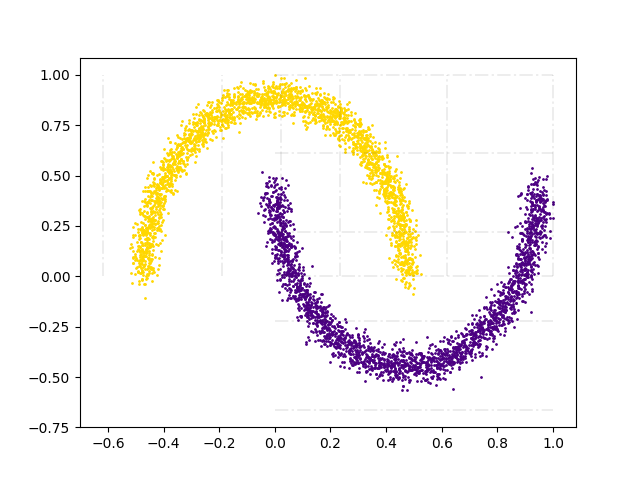
\includegraphics[width=3.5in]{img/moonsDBSCAN.png}%
\label{fig_first_case}}
\hfil
\subfloat[Clusters found by k-means.]{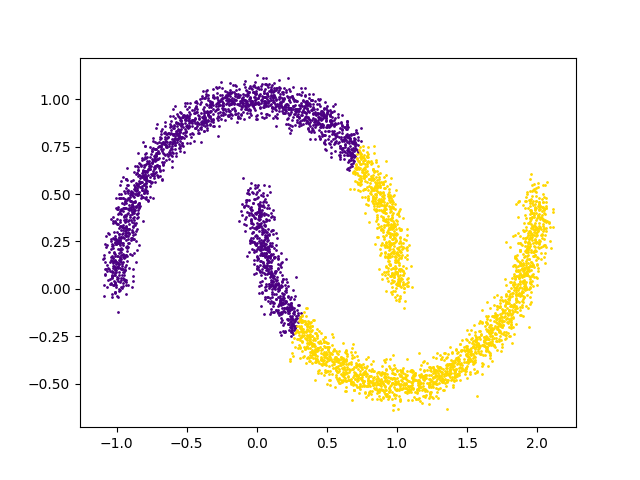
\includegraphics[width=3.5in]{img/moonsKMEANS.png}%
\label{fig_second_case}}
\caption{Comparison of the clusters provided by DBSCAN and k-means over set containing non-convex clusters.}
\label{fig_comp_clust}
\end{figure*}

\subsubsection{S.o.A for distributed implementations}

There are a variety of implementations of the DBSCAN raging from the more naive ones to more complex ones. As for comparison, a naive implementation following the exact guidelines of \cite{ReferencePaper} can be found \href{https://github.com/csegarragonz/DBSCAN-pyCOMPSs/blob/master/ext_versions/DBSCAN_Seq.py}{here}. One of the most extended and used versions programmed in \texttt{Python} is the one by \href{http://scikit-learn.org/stable/modules/generated/sklearn.cluster.DBSCAN.html}{Sklearn}.

When it comes to distributed implementations of the algorithm, most of them can be summarized in applying an efficient DBSCAN to a chunk of the dataset and using some sort of synchronization or MapReduce. This is partially the approach taken in this project but the algorithm has been reinterpreted in distributed as a whole. See for instance \href{https://github.com/bwoneill/pypardis}{this version}, an implementation using Spark.


\subsection{The framework: COMPSs} \label{compss_framework}

The \href{https://www.bsc.es/research-and-development/software-and-apps/software-list/comp-superscalar}{COMPSs} framework is a programming model designed to ease the development of applications for distributed architectures. The user programs a sequential code and defines the so-called \texttt{tasks}. The COMPSs runtime infers the dependencies and schedules the executions basing on the resources available. The model is developed in Java but has bindings for both \texttt{C} and \texttt{Python}. \texttt{PyCOMPSs} is the model chosen to develop the application. In order to mark a function as a task for the scheduler to take it into account, a small function decorator must be added. \texttt{COMPSs} is complemented by a set of tools for facilitating the monitoring and the post-mortem performance analysis (see Section \ref{performance}).

\subsection{The test zone: Mare Nostrum 4} \label{the_machine}

The Mare Nostrum 4 is the fourth generetion of supercomputers located in the \href{https://www.bsc.es}{Barcelona Supercomputing Center - Centro Nacional de Supercomputación (BSC-CNS)} its current Linpack Rmax Performance is 6.2272 Petaflops and it has been running since early July 2017. It is equipped with 48 racks with 3456 nodes. Each node has two Intel Xeon Platinum chips with 24 processors per unit.

% \begin{figure}
% \animategraphics[autoplay,controls,loop,scale=1]{3}{img/anim-}{0.png}{4.png}
% \end{figure}

\section{Implementation Proposal}
The algorithm implemented is a reinterpretation of the one exposed in \cite{ReferencePaper}, it is still though completely equivalent. The implementation can be found in \href{https://github.com/csegarragonz/DBSCAN-pyCOMPSs}{this GitHub repository}.

\subsection{Step-by-Step analysis} \label{step_by_step}

\subsubsection*{Data Pre-Processing} \label{data_pre_process}
Firstly, data is normalized by dividing each axis by the maximum value along it. This is done to prevent different factors from being really unbalanced and to ease the input parameters choice.
\begin{lstlisting}
def normalizeData(dataFile):
    """ 
    Given a dataset, divide each dimension by its maximum
    :param dataFile: path to the original .txt
    :return newName: new name of the data file containing the normalized data.
    """
\end{lstlisting}
\subsubsection*{Adaptative Partitioning} \label{partition_space} 
Secondly, the dataset is partitioned depending on the point density. Initially the three partitioning points among each axis are the minimum value, the arithmetic mean and the maximum value. Iteratively, an additional point is added in the middle of the interval containing the higher amount of points. By performing this partition, excessive unbalancing of points per square can be avoided. 
\begin{lstlisting}
def partitionSpace(dataset, fragSize, epsilon):
    """ 
    Gives a space partition basing on point density
    :returns fragData:      dict with (key,value)=(spatial id, points in the region)
    :returns rangeToEps:    list with the #squares until epsilon distance 
    """
\end{lstlisting}
Due to the theoretical possible large amount of points per cluster, an extra scale parameter is added (\texttt{numParts}), each worker will be assigned to a \texttt{numParts} part of each square resulting of the partition.
\subsubsection*{Initial Neighbor Retrieval} \label{neigh_retr} 
Once the dataset is correctly split, each worker performs a core point retrieval, please note \emph{core points} retrieval. To optimize this query, each worker knows which square he has been assigned to and consequently only looks for possible neighbors in all the adjacent squares within $\varepsilon$ distance. With this core points, a first cluster proposal is made (a cluster is a subset of the points assigned to that worker, however each worker has access to its neighbor squares points to determine whether a points neighborhood contains enough people). In the example of Figure \ref{fig_clustering}, \texttt{numParts} has been fixed to 1 so that each square is assigned to one and only one worker, otherwise intermediate results would be difficult to visually understand.
\begin{lstlisting}
def partialScan(corePoints, square, epsilon, minPoints, fragData, fragSize, numParts, rangeToEps):
    """
    Looks for all the core points (over minPoints neighbours) inside a certain square.
    :inout corePoints:  list were core points found are appended.
    :param square:      space region where core points are looked for.
    :param fragData:    dict containing space partition and its points.
    :param rangeToEps:  for each square, number of neighbors until epsilon distance. 
    """
\end{lstlisting}
\begin{figure*}[!t]
\centering
\subfloat[Dataset with adaptative partitioning.]{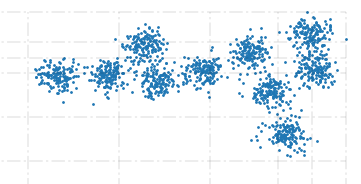
\includegraphics[width=3.5in]{img/anim-1.png}%
\label{fig_f_case}}
%\hfil
\subfloat[Initial cluster proposal.]{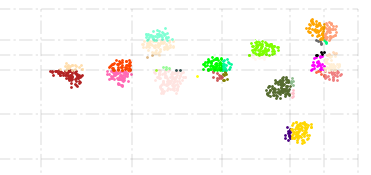
\includegraphics[width=3.5in]{img/anim-2.png}%
\label{fig_s_case}}
\hfill 
\subfloat[Clusters after synchronization.]{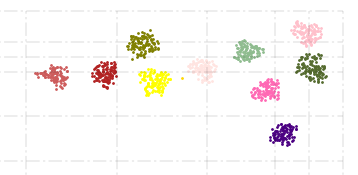
\includegraphics[width=3.5in]{img/anim-3.png}%
\label{fig_t_case}}
\hfil
\subfloat[Final output.]{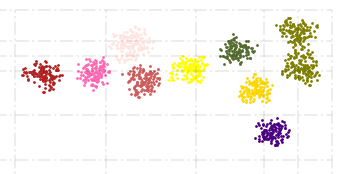
\includegraphics[width=3.5in]{img/anim-4.png}%
\label{fig_se_case}}
\caption{Plotting of the current result at each step of the algorithm.}
\label{fig_clustering}
\end{figure*}
\subsubsection*{Cluster Synchronization} \label{cluster_sync}
As a result of \ref{neigh_retr}, a huge list of clusters is obtained. To sync the corresponding results the clusters are reinterpreted as nodes in a graph and an adjacency matrix is built. The $(i,j)$-th element in the matrix will be true if and only if the distance between the $i$-th and the $j$-th cluster is lower than $\varepsilon$, see Definition \ref{def_distance}. Equivalently, each synced cluster will correspond to a connected component of the graph determined by the adjacency matrix (here a synced cluster refers to a cluster post-synchronization). Using a merge-find set, this dependencies are quickly sorted and the connected components easily found.
Since the initial number of clusters found depends on the amount of partition points chosen and on the data distribution, an extra scale parameter is introduced to prevent the algorithm of scheduling too many tasks (one per comparison). This scale parameter, $numComp$ determines how many cluster vs cluster comparisons a single task performs.
\begin{lstlisting}
def syncClusters(clusters, epsilon, numParts):
    """
    Returns a matrix of booleans. Pos [i,j]=1 <=> clusters -i and -j should be merged.
    :inout clusters:            list of all clusters and their points.
    :param numComp:             number of comparisons per worker (i.e tasks).
    :return possibleClusters:   adjacency matrix.
    """
\end{lstlisting}
\subsubsection*{Cluster Expansion} \label{cluster_exp} 
Once all the information is updated, the current result is a set of clusters of core-points.A second neighbor retrieval is performed, assigning a part of each cluster to a worker, to check for reachable points and detect possible cluster merging. Finally results are exported to a text file and, if selected, clusters are plotted and the plot saved to file.
\begin{lstlisting}
def expandCluster(clusters, fragData, epsilon, minPoints, fragSize, numParts, rangeToEps):
    """
    Expands all clusters contained in a list of clusters. 
    already established clusters.
    """
\end{lstlisting}
The whole process is summarized in Figure \ref{fig_clustering}.

\subsection{Dependency Graph}
The COMPSs framework introduced in Section \ref{compss_framework} incorporates a dependencies graph generating script, to improve the comprehension on the application behavior. 

In Figure \ref{dep_graf} two main bottlenecks in the execution can be observed (besides the last synchronization which is unavoidable). Relating to the step by step description, the first one corresponds to the initial neighbor retrieval and the first cluster proposal. One might think that this step might not need a synchronization point since the cluster vs cluster comparison does not require all the clusters to be found, just the two required to be compared. Even though this might sound true in theory, the fact that the points from a square need to be sub-partitioned again for size issues and the fact that in order to build the adjacency matrix one must know the number of nodes his graph will have make removing this synchronization point nearly impossible (at least with this implementation). However there are as well possible workarounds. For instance, a \texttt{MAX\_CLUSTS} variable could be defined and all the sizes prefixed. This goes however against one of the DBSCAN's main principle, that no information about the number of clusters is required to begin the execution. Further development on improvement proposals is exposed in Section \ref{further_development}. The second bottleneck comes after the initial cluster proposal is synced. Once we know for each cluster which cluster it can be merged too, it is mandatory to wait for all the information processed since some information might be lost and second and most important, adding points to clusters back and forth can be much more time consuming than waiting for the adjacency matrix to be fully computed and appending points only once. Both workarounds have been implemented, proving to behave worse.

\begin{figure}[!t]
\centering
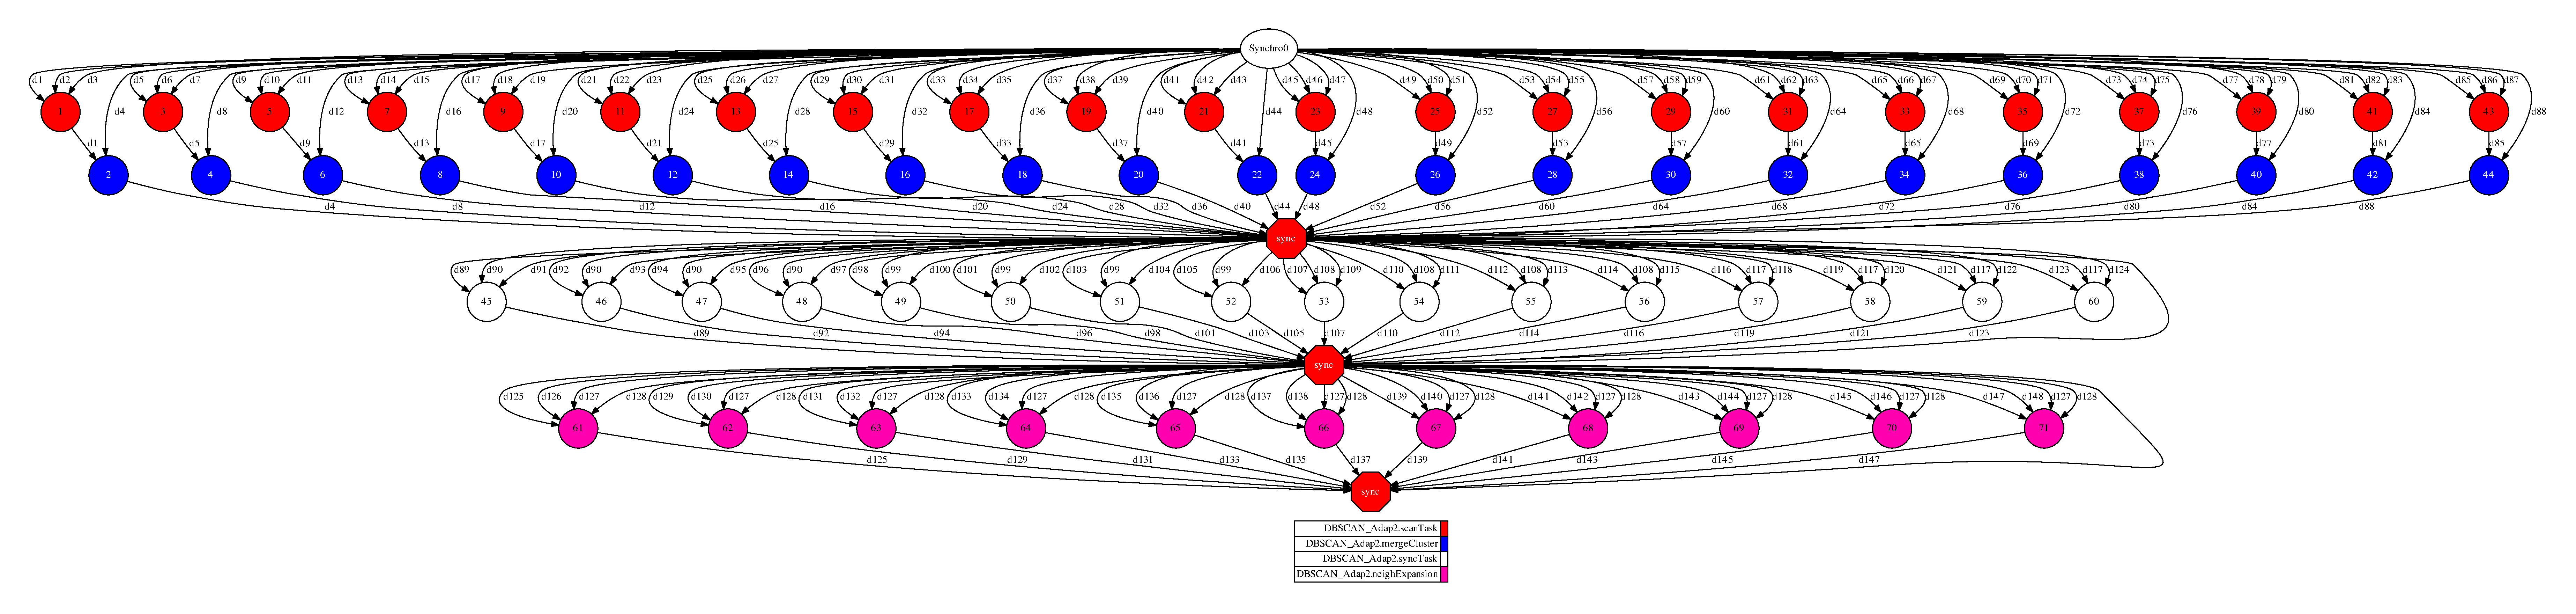
\includegraphics[width=3.5in]{img/complete_graph.pdf}
\caption{Dependency graph for a small execution.}
\label{dep_graf}
\end{figure}

\subsection{About equivalence}

Basing on the definitions given in Section \ref{the_algorithm} and the implementation exposed in Section \ref{step_by_step}. It is pretty clear that the algorithm performs completely equivalently to the one stated in \cite{ReferencePaper}. Locally at worker level, the algorithm is exactly the same, the only difference is that only a chunk of the whole dataset is used. When syncing two different situations might appear.
\begin{itemize}
\item \textbf{Clusters in different squares.} This is one of the most common situations. A natural cluster divided by the space partition performed at \ref{partition_space}. If both clusters should really be merged, then at least one point from each cluster must be at a distance lower than $\varepsilon$ and if so, the syncing process will merge them. This situation is illustrated in Figure \ref{test_case1}. Bear in mind though that after \ref{neigh_retr} only clusters of core points are found.  What if the linking point between two clusters is not a core point?
\begin{figure}[!h]
\centering
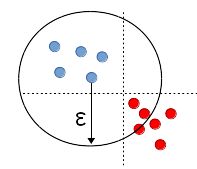
\includegraphics[width=2.5in]{img/test_case1.png}
\caption{A cluster divided by the chunking process.}
\label{test_case1}
\end{figure}
\item \textbf{Clusters related by a non-core point.} According to the reference paper, if two point-dense regions lie within a $\varepsilon$-neighborhood of the same point, even if this point might only have two neighbors, then this two clusters must be merged. In this implementation this situation is particularly fragile since initially only core points are retrieved. This dependencies are taken care off in \ref{cluster_exp}. This situation is illustrated in Figure \ref{test_case2}.
\begin{figure}[!h]
\centering
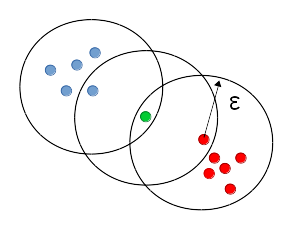
\includegraphics[width=2.5in]{img/test_case2.png}
\caption{Cluster linked by a non-core point.}
\label{test_case2}
\end{figure}
\end{itemize}

\section{Performance} \label{performance}

\subsection{Runtime Metrics}

To measure the runtime, for different dataset sizes (all three dimensional but with different number of points) the algorithm's execution time has been measured. The time measurement is performed inside the python method using the built-in tools and printed through the standard output. For the same dataset, a batch of executions with different number of workers has been performed to test the algorithm scalability. The input parameters have been modified with different data sizes but never inside the same batch of executions. Lastly all the executions have been submitted in MN4 (\ref{the_machine}) with Scratch file system. The results are summarized in Table \ref{performance_table}

\begin{table*}[!t]
\centering
\caption{Performance measured on MN4 without tracing and \texttt{fragSize}=8 and 16 CPUs per node.}
\label{performance_table}
\begin{tabular*}{.9\textwidth}{l|lc|lc|lc|lc}
 \textbf{SCRATCH}   & \textbf{NP=16} & \textbf{numComp=10} & \textbf{NP = 16} & \textbf{numComp=10} & \textbf{NP = 32} & \textbf{numComp=10} & \textbf{NP = 32} & \textbf{numComp=10} \\ \cline{2-9} 
\textbf{Workers}     & \textbf{10k}   & \textbf{Speed Up}   & \textbf{20k}     & \textbf{Speed Up}   & \textbf{50k}     & \textbf{Speed Up}   & \textbf{100k}    & \textbf{Speed Up}   \\ \hline
\textbf{1}           & 36.1205        & 1              & 125.034          & 1              & 820.14           & 1              & 3160.46          & 1              \\
\textbf{2}           & 22.47          & 1.63           & 71.66            & 1.74           & 423.36           & 1.93           & 1623.92          & 1.94           \\
\textbf{3}           & 18.05          & 2.02           & 55.043           & 2.27           & 308.014          & 2.62           & 1165.101         & 2.71           \\
\textbf{4}           & 15.916         & 2.25           & 45.609           & 2.74           & 249.59           & 3.28           & 910.3            & 3.47           \\
\textbf{5}           & 15.01          & 2.40           & 42.497           & 2.94           & 227.93           & 3.59           & 777.195          & 4.06           \\
\textbf{6}           & 14.55          & 2.48           & 40.23            & 3.16           & 196.69           & 4.16           & 703.9            & 4.48           \\
\textbf{7}           & 14.3           & 2.52           & 36.364           & 3.43           & 184              & 4.45           & 620.531          & 5.09           \\
\textbf{8}           & 13.644         & 2.64           & 33.611           & 3.72           & 171              & 4.79           & 609.211          & 5.18           \\
\textbf{16}          & 13.45          & 2.68           & 29.025           & 4.30           & 143              & 5.73           & 433.126          & 7.29           \\ \hline
\textbf{Seq} & 4690.8         &                & ---              &                & ---              &                & ---              &               
\end{tabular*}
\end{table*}

\begin{figure}[h!]
\centering	
\begin{tikzpicture}
\begin{axis}[
height=2in,
width=3.5in,
    scaled x ticks = false,
    xlabel = {\# Workers},
    grid = major,
    ylabel = {Speed Up},
    legend entries={10k, 20k, 50k, 100k}, legend style={at={(0.05,-0.25)},anchor=north west, draw=none, legend columns=-1}
    %xtick={0.028503, 0.0427553,0.0570},
    %xticklabels={$l-2\lambda$, $l-\lambda$,$l$},
    %ytick={0,1,2},
    %yticklabels={0,$|E_{0i}|$,$2|E_{0i}|$},
]
\addplot[mark=o, thick, blue] table {data/10k.dat};
\addplot[mark=o, thick, orange] table {data/20k.dat};
\addplot[mark=o, thick, red] table {data/50k.dat};
\addplot[mark=o, thick, green] table {data/100k.dat};
%Here the blue parabloa is defined
\end{axis}
\end{tikzpicture}
\caption{Speed Up as a function of the number of workers for different datasets.}
\label{speed_up}
\end{figure}

In figure \ref{speed_up} the speed up vs number of workers is plotted. To understand why it increases as the number of points increases check section \ref{q_coi_passa}. In addition to that, a runtime vs number of workers plot can be found at \ref{rt_plot}.

\begin{figure}[h!]
\centering	
\begin{tikzpicture}
\begin{axis}[
height=2in,
width=3.5in,
    scaled x ticks = false,
    xlabel = {\# Workers},
    grid = major,
    ylabel = {Execution Time},
    legend entries={10k, 20k, 50k, 100k}, legend style={at={(0.05,-0.25)},anchor=north west, draw=none, legend columns=-1}
    %xtick={0.028503, 0.0427553,0.0570},
    %xticklabels={$l-2\lambda$, $l-\lambda$,$l$},
    %ytick={0,1,2},
    %yticklabels={0,$|E_{0i}|$,$2|E_{0i}|$},
]
\addplot[mark=o, thick, blue] table {data/10kRT.dat};
\addplot[mark=o, thick, orange] table {data/20kRT.dat};
\addplot[mark=o, thick, red] table {data/50kRT.dat};
\addplot[mark=o, thick, green] table {data/100kRT.dat};
%Here the blue parabloa is defined
\end{axis}
\end{tikzpicture}
\caption{Execution time as a function of the number of workers for different datasets.}
\label{rt_plot}
\end{figure}

\subsection{Critical Analysis} \label{critical_analysis}

\subsubsection*{Dependence on the scale parameters:}

From the explanation in Section \ref{the_algorithm} it is easy to see that the paradigm has shifted from a two parameter algorithm to a four one. In the one hand this enables, when run with knowledge, the algorithm to adapt better to mutable resources and data loads. In the other hand this also increases the variability of the performance and may be a drawback at some points.

Emphasizing on this two extra parameters, one of them has not got a clear impact on the runtime metrics. The number of comparisons executed by a worker, \texttt{numComp} will determine a certain type of task's length but won't increase their variability. However, \texttt{numParts} chunks the data again having a direct effect on the number of clusters initially found and consequently on the number of tasks performed at the syncing stage. In addition to that, it reduces the average task duration but at the same time makes tasks less homogeneous. This process causes bigger executions (more points and assigned nodes) to behave less homogeneously. In spite of that, this scale parameter is necessary to ensure the algorithm scalability, otherwise this would depend entirely on the data distribution.

\begin{figure}[!h]
\centering
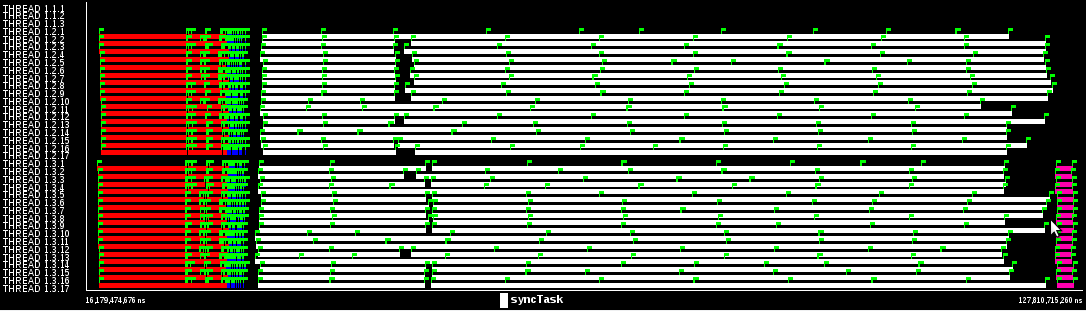
\includegraphics[width=3.5in]{img/traca_compacte.png}
\caption{Tracing with 10k points and $\texttt{numParts}=16$.}
\label{traca_bona}
\end{figure}

To dig in this sections where the algorithm is not behaving as expected, or at least not as desired, a performance analysis using tracing (\href{https://tools.bsc.es/paraver}{Paraver}) is performed. In Figure \ref{traca_bona} there is an example of a small execution with  $\texttt{numParts}=16$ and 10000 points. Consequently with the above lines, a homogeneous trace is obtained. In Figure \ref{traca_caca} the opposite behavior is exposed. For this second execution the number of points was around 20000 and $\texttt{numParts}=32$. It is easy to see that tasks duration becomes much more volatile (green flags indicate a task' beginning and ending) and they are not so easily scheduled.

\begin{figure}[!h]
\centering
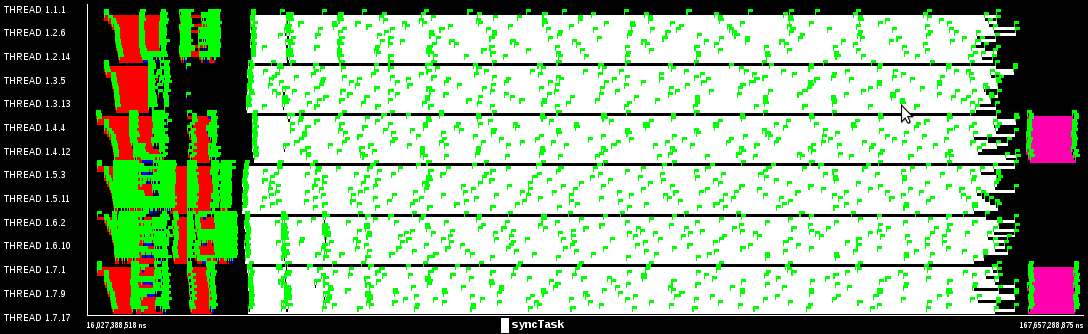
\includegraphics[width=3.5in]{img/traca_mes_caca.png}
\caption{Tracing with 20k points and $\texttt{numParts}=32$.}
\label{traca_caca}
\end{figure}

\subsubsection*{On memory, CPUs per node and scalability:} \label{q_coi_passa}

Another issue faced when testing the algorithm is the memory vs cpu per node paradigm. Initially each node at \ref{the_machine} has 2GB of memory , however if the user requests for less workers and exclusivity each node will have more memory since the whole batch is divided between the running cores. When the dataset tends to be bigger and bigger, the memory requested is bigger as well. Hence the performance at some points might be better with less \texttt{cpus\_per\_node} in spite of the time lost with inter-node communication. 

\section{Conclusion}

Following along the reasoning from \ref{critical_analysis}, the algorithm is really sensitive to changes in the input parameters. Thus this parameters should somehow depend on the resources available, however that would make the algorithm not structure-unaware. This might be one of the reasons why scalability and speed up is not exactly as desired since all the tests for the same dataset are performed under the same input parameters (to be able to compare them). Therefore the theoretical speedup might decrease in comparison to if we were to run the algorithm manually test by test.

\subsection{Further Development and Improvement Proposals} \label{further_development}
The main development I would recommend implementing would be a smart guessing at execution time of the scale parameters. Empirically it has been proven that if the user is able to choose the right parameters, the algorithm is going to have a great performance. As a consequence, being able to guess them at execution time would guarantee a stability that for this moment I can not ensure.

Secondly, the DBSCAN method could be expanded to a generalized DBSCAN to detect arbitrary cluster densities removing the dependencies to the input parameters, \texttt{minPoints} and $\varepsilon$.

Lastly and in the opposite direction of the second proposal, some research into parallel optimization models so to guess the input parameters (rather than using a thumb rule) could be done.


\begin{thebibliography}{1}
\bibitem{ReferencePaper}
Ester, Martin Kriegel, Hans-Peter Sander, Jorg Xu, Xiaowei (1996). \textit{A density-based algorithm for discovering clusters in large spatial databases with noise.} Proceedings of the Second International Conference on Knowledge Discovery and Data Mining (KDD-96)
\end{thebibliography}

\end{document}


